%% Преамбула TeX-файла

% 1. Стиль и язык
\documentclass[utf8x, 12pt]{G7-32} % Стиль (по умолчанию будет 14pt)

% Остальные стандартные настройки убраны в preamble.inc.tex.
\sloppy

% Настройки стиля ГОСТ 7-32
% Для начала определяем, хотим мы или нет, чтобы рисунки и таблицы нумеровались в пределах раздела, или нам нужна сквозная нумерация.
\EqInChapter % формулы будут нумероваться в пределах раздела
\TableInChapter % таблицы будут нумероваться в пределах раздела
\PicInChapter % рисунки будут нумероваться в пределах раздела
\usepackage{slashbox}

% Добавляем гипертекстовое оглавление в PDF
\usepackage[
bookmarks=true, colorlinks=true, unicode=true,
urlcolor=black,linkcolor=black, anchorcolor=black,
citecolor=black, menucolor=black, filecolor=black,
]{hyperref}

% Изменение начертания шрифта --- после чего выглядит таймсоподобно.
% apt-get install scalable-cyrfonts-tex

\IfFileExists{cyrtimes.sty}
    {
        \usepackage{cyrtimespatched}
    }
    {
        % А если Times нету, то будет CM...
    }

\usepackage{graphicx}   % Пакет для включения рисунков

% С такими оно полями оно работает по-умолчанию:
% \RequirePackage[left=20mm,right=10mm,top=20mm,bottom=20mm,headsep=0pt]{geometry}
% Если вас тошнит от поля в 10мм --- увеличивайте до 20-ти, ну и про переплёт не забывайте:
\geometry{right=20mm}
\geometry{left=30mm}


% Пакет Tikz
\usepackage{tikz}
\usetikzlibrary{arrows,positioning,shadows}

% Произвольная нумерация списков.
\usepackage{enumerate}

% ячейки в несколько строчек
\usepackage{multirow}

% itemize внутри tabular
\usepackage{paralist,array}
\usepackage[utf8]{inputenc}


% Центрирование подписей к плавающим окружениям
\usepackage[justification=centering]{caption}


% Настройки листингов.
\ifPDFTeX
% 8 Листинги

\usepackage{listings}
\usepackage{wrapfig}
% Значения по умолчанию
\lstset{
  basicstyle= \footnotesize,
  breakatwhitespace=true,% разрыв строк только на whitespacce
  breaklines=true,       % переносить длинные строки
%   captionpos=b,          % подписи снизу -- вроде не надо
  inputencoding=koi8-r,
  numbers=left,          % нумерация слева
  numberstyle=\footnotesize,
  showspaces=false,      % показывать пробелы подчеркиваниями -- идиотизм 70-х годов
  showstringspaces=false,
  showtabs=false,        % и табы тоже
  stepnumber=1,
  tabsize=4,              % кому нужны табы по 8 символов?
  frame=single,
  literate={а}{{\selectfont\char224}}1
  {б}{{\selectfont\char225}}1
  {в}{{\selectfont\char226}}1
  {г}{{\selectfont\char227}}1
  {д}{{\selectfont\char228}}1
  {е}{{\selectfont\char229}}1
  {ё}{{\"e}}1
  {ж}{{\selectfont\char230}}1
  {з}{{\selectfont\char231}}1
  {и}{{\selectfont\char232}}1
  {й}{{\selectfont\char233}}1
  {к}{{\selectfont\char234}}1
  {л}{{\selectfont\char235}}1
  {м}{{\selectfont\char236}}1
  {н}{{\selectfont\char237}}1
  {о}{{\selectfont\char238}}1
  {п}{{\selectfont\char239}}1
  {р}{{\selectfont\char240}}1
  {с}{{\selectfont\char241}}1
  {т}{{\selectfont\char242}}1
  {у}{{\selectfont\char243}}1
  {ф}{{\selectfont\char244}}1
  {х}{{\selectfont\char245}}1
  {ц}{{\selectfont\char246}}1
  {ч}{{\selectfont\char247}}1
  {ш}{{\selectfont\char248}}1
  {щ}{{\selectfont\char249}}1
  {ъ}{{\selectfont\char250}}1
  {ы}{{\selectfont\char251}}1
  {ь}{{\selectfont\char252}}1
  {э}{{\selectfont\char253}}1
  {ю}{{\selectfont\char254}}1
  {я}{{\selectfont\char255}}1
  {А}{{\selectfont\char192}}1
  {Б}{{\selectfont\char193}}1
  {В}{{\selectfont\char194}}1
  {Г}{{\selectfont\char195}}1
  {Д}{{\selectfont\char196}}1
  {Е}{{\selectfont\char197}}1
  {Ё}{{\"E}}1
  {Ж}{{\selectfont\char198}}1
  {З}{{\selectfont\char199}}1
  {И}{{\selectfont\char200}}1
  {Й}{{\selectfont\char201}}1
  {К}{{\selectfont\char202}}1
  {Л}{{\selectfont\char203}}1
  {М}{{\selectfont\char204}}1
  {Н}{{\selectfont\char205}}1
  {О}{{\selectfont\char206}}1
  {П}{{\selectfont\char207}}1
  {Р}{{\selectfont\char208}}1
  {С}{{\selectfont\char209}}1
  {Т}{{\selectfont\char210}}1
  {У}{{\selectfont\char211}}1
  {Ф}{{\selectfont\char212}}1
  {Х}{{\selectfont\char213}}1
  {Ц}{{\selectfont\char214}}1
  {Ч}{{\selectfont\char215}}1
  {Ш}{{\selectfont\char216}}1
  {Щ}{{\selectfont\char217}}1
  {Ъ}{{\selectfont\char218}}1
  {Ы}{{\selectfont\char219}}1
  {Ь}{{\selectfont\char220}}1
  {Э}{{\selectfont\char221}}1
  {Ю}{{\selectfont\char222}}1
  {Я}{{\selectfont\char223}}1
}

% Стиль для псевдокода: строчки обычно короткие, поэтому размер шрифта побольше
\lstdefinestyle{pseudocode}{
  basicstyle=\small,
  keywordstyle=\color{black}\bfseries\underbar,
  language=Pseudocode,
  numberstyle=\footnotesize,
  commentstyle=\footnotesize\it
}

% Стиль для обычного кода: маленький шрифт
\lstdefinestyle{realcode}{
  basicstyle=\scriptsize,
  numberstyle=\footnotesize
}

% Стиль для коротких кусков обычного кода: средний шрифт
\lstdefinestyle{simplecode}{
  basicstyle=\footnotesize,
  numberstyle=\footnotesize
}

% Стиль для BNF
\lstdefinestyle{grammar}{
  basicstyle=\footnotesize,
  numberstyle=\footnotesize,
  stringstyle=\bfseries\ttfamily,
  language=BNF
}

% Определим свой язык для написания псевдокодов на основе Python
\lstdefinelanguage[]{Pseudocode}[]{Python}{
  morekeywords={each,empty,wait,do},% ключевые слова добавлять сюда
  morecomment=[s]{\{}{\}},% комменты {а-ля Pascal} смотрятся нагляднее
  literate=% а сюда добавлять операторы, которые хотите отображать как мат. символы
    {->}{\ensuremath{$\rightarrow$}~}2%
    {<-}{\ensuremath{$\leftarrow$}~}2%
    {:=}{\ensuremath{$\leftarrow$}~}2%
    {<--}{\ensuremath{$\Longleftarrow$}~}2%
}[keywords,comments]

% Свой язык для задания грамматик в BNF
\lstdefinelanguage[]{BNF}[]{}{
  morekeywords={},
  morecomment=[s]{@}{@},
  morestring=[b]",%
  literate=%
    {->}{\ensuremath{$\rightarrow$}~}2%
    {*}{\ensuremath{$^*$}~}2%
    {+}{\ensuremath{$^+$}~}2%
    {|}{\ensuremath{$|$}~}2%
}[keywords,comments,strings]

% Подписи к листингам на русском языке.
\renewcommand\lstlistingname{\cyr\CYRL\cyri\cyrs\cyrt\cyri\cyrn\cyrg}
\renewcommand\lstlistlistingname{\cyr\CYRL\cyri\cyrs\cyrt\cyri\cyrn\cyrg\cyri}

\else
\usepackage{local-minted}
\fi

% Полезные макросы листингов.
% Любимые команды
\newcommand{\Code}[1]{\textbf{#1}}


\begin{document}

\frontmatter % выключает нумерацию ВСЕГО; здесь начинаются ненумерованные главы: реферат, введение, глоссарий, сокращения и прочее.

% Команды \breakingbeforechapters и \nonbreakingbeforechapters
% управляют разрывом страницы перед главами.
% По-умолчанию страница разрывается.

% \nobreakingbeforechapters
% \breakingbeforechapters

% Также можно использовать \Referat, как в оригинале
%\begin{abstract}
%	Титульный лист. Эта страница нужна мне, чтобы не сбивалась нумерация страниц
%	\cite{Dh}
%	\cite{Bayer}
%	\cite{Habr1}
%	\cite{Noise_func}
%	\cite{Ulich}

%Это пример каркаса расчётно-пояснительной записки, желательный к использованию в РПЗ проекта по курсу РСОИ.

%Данный опус, как и более новые версии этого документа, можно взять по адресу (\url{https://github.com/rominf/latex-g7-32}).

%Текст в документе носит совершенно абстрактный характер.
%\end{abstract}
% НАЧАЛО ТИТУЛЬНОГО ЛИСТА
\begin{center}
	\hfill \break
	\textit{
		\normalsize{Государственное образовательное учреждение высшего профессионального образования}}\\ 
	
	\textit{
		\normalsize  {\bf  «Московский государственный технический университет}\\ 
		\normalsize  {\bf имени Н. Э. Баумана»}\\
		\normalsize  {\bf (МГТУ им. Н.Э. Баумана)}\\
	}
	\noindent\rule{\textwidth}{2pt}
	\hfill \break
	\noindent
	\makebox[0pt][l]{ФАКУЛЬТЕТ}%
	\makebox[\textwidth][c]{«Информатика и системы управления»}%
	\\
	\noindent
	\makebox[0pt][l]{КАФЕДРА}%
	\makebox[\textwidth][r]{«Программное обеспечение ЭВМ и информационные технологии»}%
	\\
	\hfill\break
	\hfill \break
	\hfill \break
	\hfill \break
	\normalsize{\bf Р А С Ч Ё Т Н О - П О Я С Н И Т Е Л Ь Н А Я\space\space З А П И С К А}\\
	\normalsize{\bf к курсовой работе на тему:}\\
	\hfill \break
	\large{Реализации инструмента анализа параллельных программ}\\
	\hfill \break
	\hfill \break
	\hfill \break
	\hfill \break
	\hfill \break	
	\normalsize {
		\noindent
		\makebox[0pt][l]{Студент}%
		\makebox[\textwidth][c]{Капустин А.И.}%
		\makebox[0pt][r]{{$\underset{\text{(Подипсь, дата)}}{\underline{\hspace{8cm}}}$ \space И.О. Фамилия}}
	}\\
	\hfill \break	
	\normalsize {
		\noindent
		\makebox[0pt][l]{Руководитель курсового проекта}%
		\makebox[\textwidth][c]{ ~~~~~~~~      Ковтушенко А.П.}%
		\makebox[0pt][r]{{$\underset{\text{(Подпись, дата)}}{\underline{\hspace{6cm}}}$ \space И.О. Фамилия}}
	}
	\hfill \break
	\hfill \break
	\hfill \break
	\hfill \break
\end{center}
\hfill \break
\hfill \break
\begin{center} Москва 2017 \end{center}

\thispagestyle{empty} % 
% КОНЕЦ ТИТУЛЬНОГО ЛИСТА


%%% Local Variables: 
%%% mode: latex
%%% TeX-master: "rpz"
%%% End: 

\tableofcontents


%%% Local Variables:
%%% mode: latex
%%% TeX-master: "rpz"
%%% End:

%
%%% Local Variables:
%%% mode: latex
%%% TeX-master: "rpz"
%%% End:


\Introduction

Вычислительные системы с массовым параллелизмом совершили революцию в мире параллельных вычислений, обеспечив производительность порядка нескольких Терафлоп/с. Необходимость в вычислениях такого объёма возникает в широком круге областей от молекулярной физики до предсказания погоды. На сегодняшний день массивно параллельные системы являются лидерами по критерию цена/производительность.
Однако, за таким прогрессом аппаратного обеспечения не поспевало программное обеспечение. Очевидно, что будут созданы более мощные массивно параллельные системы, и основной проблемой становится разработка программного обеспечения, способного максимально использовать вычислительные ресурсы. Параллельные вычисления связаны с очень сложным и тяжело понимаемым ходом выполнения программ, и недостаточно полное понимание не позволяет полностью использовать вычислительные ресурсы.
Так как производительность – самый важный критерий при использовании параллельных компьютеров, и так как производительность пилотных реализаций параллельных программ как правило далека от ожидаемой, модификация программы с целью повышения производительности является важной частью процесса разработки. Основным фактором, ведущим к большому количеству трудоёмкой работы, требующей высокой квалификации является нехватка средств для анализа и оценки производительности. При отсутствии таких средств, причины низкой производительности выявляются с помощью средств, разработанных для конкретного приложения и метода тыка. Повышение производительности параллельных программ наиболее важная, но трудоёмкая задача, которая требует хорошего понимания задачи. Цель средств контроля и визуализации производительности параллельных программ – помочь разработчику обрести это понимание.
Визуализация производительности заключается в использовании графических образов для представления анализа данных о выполнении программы для лучшего её понимания. Такие средства визуализации были очень полезны и в прошлом, и широко используются в настоящее время для повышения производительности параллельных программ. Несмотря на прогресс в области визуализации научных данных, технологии визуализации для параллельного программирования являются объектом внимания многих разработчиков, так как требуется тем более сложная визуализация, чем более сложными становятся параллельные системы.


\mainmatter % это включает нумерацию глав и секций в документе ниже

\chapter{Аналитический раздел}
\label{cha:analysis}
%
% % В начале раздела  можно напомнить его цель
%
Алгоритмы, с которыми приходится иметь дело при параллельном программировании гораздо сложнее, чем аналогичные последовательные алгоритмы. Часть проблем касается распараллеливания самого алгоритма (например, как разбить процесс на задачи и как поставить им в соответствие физические процессоры), часть касается оптимального использования вычислительных ресурсов (баланс загрузки процессоров, межпроцессные взаимодействия, доступ к кэшу). Для разработки высокопроизводительных приложений программисту не только очень хорошо знать структуру самого приложения, но и структуру аппаратной платформы, а зачастую и программной (особенности операционной системы, компилятора и.т.д.).
Итак, уровень знаний, необходимый для разработки высокопроизводительных параллельных программ выше, чем для последовательных программ. Параллельное программирование может быть очень мучительным и запутанным. Вдобавок отладка параллельной программы и поиск критических мест также трудоёмкий и длительный процесс.
Из-за этих причин программирование для массивно параллельных машин считается непростым делом, и в значительной степени причиной этому служит недостаток инструментария по сравнению с последовательными машинами. Для того, чтобы понять поведение и внутреннюю логику параллельных программ и помочь программисту выявить потенциальные слабые места (например, ограничения по межпроцессным взаимодействиям) необходимы средства контроля хода выполнения параллельной программы. Они могут использоваться для сравнения производительности схожих программ или помогать при отладке.


% Обратите внимание, что включается не ../dia/..., а inc/dia/...
% В Makefile есть соответствующее правило для inc/dia/*.pdf, которое
% берет исходные файлы из ../dia в этом случае.



\section{Парадигмы параллельного программирования}
\subsection{Структура и характеристики параллельных алгоритмов}
Любой параллельный алгоритм (программа) состоит из блоков последовательных и параллельных вычислений. Последовательная часть программы (называется критическим сечением) – это последовательность операторов, которая должна выполняться только одним процессором. За критическим сечением обычно следует ветвление, инициирующее параллельно выполняемые участки программы (параллельные сегменты). В месте соединения параллельных сегментов выполняется синхронизация и параллельные сегменты возвращаются к критическому сечению. Синхронизация требуется для того, чтобы вычисления в параллельных сегментах закончились прежде, чем начнется выполнение последовательной части. 

\subsection{Программные парадигмы}

При параллельном программировании появляются дополнительные сложности (по сравнению с последовательным программированием): возникает необходимость управлять несколькими процессорами и координировать межпроцессорные вызовы. В общем случае параллельная программа представляет собой ряд заданий, работающих параллельно друг другу и взаимодействующих между собой. Существует несколько парадигм (моделей) программирования при создании параллельных алгоритмов. Наиболее распространенными парадигмами являются модель передачи сообщений и модель разделяемой памяти.


\subsection{Проектирование параллельных алгоритмов}
Несмотря на то, что проектирование параллельных алгоритмов есть процесс творческий и в общем случае достаточно сложно рекомендовать универсальный рецепт, следует все же привести общую методологию проектирования параллельных алгоритмов, которая в значительной степени оградит проектировщика от потенциальных ошибок.

\begin{figure}[h!]
	\centering
	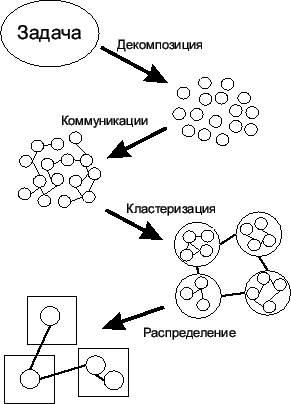
\includegraphics[width=0.4\textwidth]{img/img1.png}
	\caption{Методология проектирования параллельных алгоритмов}
	\label{fig:spire05}
\end{figure}

Описываемая методология проектирования предлагает подход к распараллеливанию, который рассматривает машинно-независимые аспекты реализации алгоритма, такие как параллелизм, на первой стадии, а особенности проектирования, связанные с конкретным параллельным компьютером, - на второй. Данный подход разделяет процесс проектирования на четыре отдельных этапа: декомпозиция (partitioning), коммуникации (communications), кластеризация (agglomeration) и распределение (mapping). Первые два этапа призваны выделить в исходной задаче параллелизм и масштабируемость, остальные этапы связаны с различными аспектами производительности алгоритма\cite{test1_B}. Рисунок 1.1 иллюстрирует процесс проектирования параллельного алгоритма.  
Сформулируем кратко содержание этих этапов. 
\subsubsection{Декомпозиция} 
Общая задача вычислений и обработки данных делится на меньшего размера подзадачи. При этом игнорируются проблемы практической реализации, например, число процессоров используемого в будущем компьютера. Напротив, все внимание сосредотачивается на возможном параллелизме исходной задачи. 
\subsubsection{Коммуникации}
Определяется требуемая связь между подзадачами, ее структура и конкретные алгоритмы коммуникаций. 
\subsubsection{Кластеризация} 
Структура подзадач и коммуникаций оценивается с учетом требований производительности алгоритма и затрат на реализацию. Если необходимо, отдельные подзадачи комбинируются в более крупные с целью улучшения производительности и снижения затрат на разработку. 
\subsubsection{Распределение} 
Каждая подзадача назначается определенному процессору, при этом стараются максимально равномерно загрузить процессоры и минимизировать коммуникации. Распределение может быть статическим или формироваться в процессе выполнения программы на основе алгоритмов балансировки загрузки (load balancing algorithms). 
Следует заметить, что при прохождении последних двух этапов необходимо учитывать архитектуру параллельного компьютера, имеющегося в распоряжении разработчика, другими словами параллельный алгоритм должен быть адекватен используемой параллельной системе. 

\subsection{Характеристики производительности параллельного алгоритма}
Задачей программиста является проектирование и реализация программ, которые удовлетворяют требованиям пользователя в смысле производительности и корректной работы. Производительность является достаточно сложным и многосторонним понятием. Кроме времени выполнения программы и масштабируемости следует также анализировать механизмы, отвечающие за генерацию, хранение и передачу данных по сети, оценивать затраты, связанные с проектированием, реализацией, эксплуатацией и сопровождением программного обеспечения. Существуют весьма разнообразные параметры, влияющие на производительность вычислительной системы. Среди них наиболее значимыми являются: требования по памяти, производительность сети, время задержки при передаче данных (latency time), переносимость, масштабируемость, затраты на проектирование, реализацию, отладку, требование к аппаратному обеспечению и т.д. Критериями, по которым оценивается производительность, являются время выполнения программы, ускорение и эффективность.
Относительная важность различных параметров будет меняться в  зависимости от природы вычислительной системы и поставленной задачи. Специфика конкретной задачи может требовать высоких показателей для каких-либо определенных критериев, в то время как остальные должны быть оптимизированы или полностью игнорированы. 
Ниже мы рассмотрим лишь две характеристики производительности, а именно, эффективность и ускорение, поскольку они наиболее часто используются при анализе производительности параллельных алгоритмов.
\subsubsection{Ускорение и эффективность}
Ускорение параллельного алгоритма $S_{p}$ определяется следующим образом:
\begin{equation}
S_{p0}=\frac{T_{0} }{T_{p}} \\
\label{F:100}
\end{equation}
\begin{equation}
S_{p}=\frac{T_{1} }{T_{p}}
\label{F:101}
\end{equation}
где $T_{0}$- время работы наилучшего последовательного алгоритма, $T_{1}$ -- время работы параллельного алгоритма на одном процессоре, $T_{p}$ -- время работы параллельного алгоритма на p процессорах.Следует отметить, что в общем случае T0<T1, т.е. последовательный алгоритм работает быстрее, чем параллельный алгоритм с использованием одного процессора, т.к. в любом параллельном алгоритме всегда присутствует дополнительная часть кода, обеспечивающая распараллеливание вычислений, а именно точки синхронизации, передача данных от одного процессора к другому и т.д. Кроме того, наиболее оптимальные алгоритмические решения не всегда хорошо параллелизуются. Таким образом, при анализе ускорения алгоритма следует всегда оговаривать, какое из определений используется \cite{book2}. 
В общем случае редко удается полностью распараллелить вычислительный процесс и получить максимальное ускорение в p раз. и один параллельный алгоритм не может обеспечить идеальную балансировку нагрузки процессоров, т.е. в равной степени разделить вычислительную работу между процессорами. Эффективность $E_{p}$ параллельного алгоритма характеризует степень загрузки процессоров и определяется как отношение ускорения $S_{p}$ к максимально возможному ускорению p:
\begin{equation}
E_{p}=\frac{S_{p} }{p}
\label{F:102}
\end{equation}
Нетрудно заметить, что
\begin{equation}
1\leq S_{p} \leq p,\; \;  \frac{1}{p} \leq E_{p} \leq 1
\label{F:103}
\end{equation}
\subsubsection{Закон Амдала}
Пусть $\alpha\leq 1$ есть некая доля вычислений, которые выполняются в параллельном режиме, а доля $1-\alpha$  – в последовательном без совмещения этих режимов во времени. Тогда последовательные вычисления занимают время $(1-\alpha)T$ , a параллельные – время $\frac{\alpha T_{1}}{p}\;$. Оба режима занимают время $T_{p}T_{1}(1-\alpha+\frac{\alpha}{p})$.
Тогда формулы для ускорения $S_{p}$ (\ref{F:101}) и эффективности  $E_{p}$ (\ref{F:102}) принимают вид:
\begin{equation}
S_{p}=\frac{p}{p-\alpha(p-1)}
\label{F:104}
\end{equation}
\begin{equation}
E_{p}=\frac{1-\alpha}{(1-\alpha)p +\alpha}
\label{F:105}
\end{equation} 
Формулы (\ref{F:104})  и (\ref{F:105}) и выражают простую и обладающую большой общностью зависимость, известную как закон Амдала. Согласно этому закону в алгоритме, имеющем два не совмещенных во времени режима последовательных и параллельных вычислений, при  $n\to\infty $ границу ускорения составляет величина, обратная доле последовательных вычислений:
\begin{equation}
\lim_{x \to \infty} \left(S_{p} \right) = \frac{1}{1-\alpha} 
\label{F:106}
\end{equation} 
\begin{figure}[h!]
	\centering
	
\includegraphics[width=0.45\textwidth]{img/img2.png}
	
\includegraphics[width=0.45\textwidth]{img/img3.png}
	\caption{Зависимость ускорения $S_{p}$ от числа процессоров p для различных объемов параллельных вычислений $\alpha$ (слева) и от объема параллельных вычислений($\alpha$)  для различного числа процессоров p (справа).}
	\label{fig:spire06}
\end{figure}
\begin{figure}[h!]
	\centering
	
\includegraphics[width=0.45\textwidth]{img/img4.png}

	\caption{Зависимость эффективности $E_{p}$от объема параллельных вычислений $\alpha$ для различного числа процессоров p.}
	\label{fig:spire07}
\end{figure}
Для повышения скорости вычислений за счет распараллеливания требуется повышать скорость параллельных вычислений, однако остающиеся последовательные вычисления все в большей степени тормозят ускорение в целом. Даже небольшая доля последовательных вычислений может сильно снизить общую скорость. 
Особенно сильное влияние на ускорение и эффективность алгоритма последовательные вычисления оказывают в области $\alpha$ , близкому к 1. Поэтому в алгоритмах с большим объемом параллельных вычислений заметным является уменьшение последовательных вычислений даже на доли процента от общего объема вычислений. 
Закон Амдала представляет собой приближенную модель ускорения, т.к. не учитывает так называемые накладные расходы и зависимость $\alpha$ от p. Однако в общем случае доля параллельных вычислений может меняться с изменением числа используемых процессоров (проблема масштабируемости).


\subsubsection{Факторы, снижающие ускорение }
Факторы, снижающие ускорение (overheads)
К основным факторам, приводящим к снижению ускорения, относятся: 
\begin{enumerate}
\item Разбалансировка нагрузки процессоров (load unbalancing). Неравномерная распределение вычислительной работы между процессорами - отдельные процессоры могут простаивать (idle processors) - не обеспечивает высокой степени параллелизма, что в свою очередь снижает эффективность; 
\item Синхронизация процессоров (processor synchronization). На выполнение программного кода, обеспечивающего синхронизацию типа барьер, требуются временные затраты. 
\item Коммуникации (communications). При обмене сообщениями между процессорами могут возникать задержки как вследствие особенностей программной реализации алгоритма (например, на момент принятия сообщения процессором оно еще не отправлено другим процессором), так и вследствие аппаратных причин (например, загруженность сети). 
\item Параллельный ввод/вывод (parallel input/output). Например, программы, работащие на различных процессорах, одновременно выводят данные в один и тот же файл и т.д. 
\end{enumerate}
\subsection{Наблюдение за выполнением параллельной программы}
Практика показывает, что производительность параллельной программы далеко не всегда растёт с ростом мощности используемого аппаратного обеспечения. Причин этому много: пользователи хотят видеть более удобные сервисы системы, потребляющие вычислительную мощь, механизмы обеспечения безопасности также требуют процессорного времени. От этих эффектов невозможно избавиться.
Со стороны разработчика эффективность использования вычислительных ресурсов может быть увеличена за счёт тщательной разработки программных продуктов с одной стороны и анализа поведения программ во время выполнения – с другой. Если анализ производительности является важным для последовательных программ, то для параллельных и распределённых систем он жизненно необходим. Причиной этому служат сложные взаимодействия между разными частями программы, работающими над решением одной общей задачи.
Необходимость использования общих ресурсов ведёт к проблемам связанными с синхронизацией процессов, временем ожидания, тупиками и т.д. Кроме обычных проблем последовательной программы возникают новые трудности, связанные с управлением параллельными задачами, которые влекут к потере процессорной мощности, тем самым  процессорная мощность не используется на том уровне, на котором могла.
Наблюдение за ходом выполнения программы, с помощью событийного подхода, ведёт к большим объёмам файлов трасс. Для того чтобы сконцентрироваться на местах трассы, представляющих интерес, необходимо выявить их местоположение. Следовательно, для общего и быстрого анализа необходимо использовать статистические методы. После получения такой информации, можно применять более детальный подход. При этом частой задачей является не только измерение производительности системы или её части, но и получение представления о динамическом взаимодействии процессов.
\subsubsection{Проблемы производительности параллельных систем}
Настройка последовательных программ относительно проста: используется профилирование для определения наиболее часто используемых частей. Обычно, это лишь малая часть всего кода. Переработка этих частей программы приводит к увеличению производительности. Этот простой подход не работает в случае параллельных и распределённых программ. Например, оптимизация части программы, которая должна ждать промежуточного результата счёта другого процесса, не принесёт выгоды – этот процесс просто будет находиться в состоянии ожидания больше времени. Для того, чтобы определить почему программа ведёт себя так, как она себя ведёт, надо искать причины такого поведения. Это ведёт к рассмотрению причинно-следственных связей в системе. Как будет показано далее, анализ параллельной системы с этой токи зрения может привести к интересным результатам.
\subsubsection{Детерминированность компьютерных системы}
В общих чертах, детерминированность представляет собой закон, по которому определённое действие ведет к определённому результату. В контексте вычислительных систем детерминированность означает, что поведение процессов определяется законом, выраженным в виде программы. То есть будущее каждого процесса зависит от текущего положения в программе, текущего контекста относительно других процессов и следующей инструкции программы. Есть несколько специфичных вопросов, относящихся к параллельным системам. В последовательных программах инструкции выполняются в том же порядке, как и в тексте программы, за исключением ветвлений. В этом случае следующая инструкция определяется исходя их некоторых условий. Рассматривая все инструкции как потенциальные события, каждая не управляющая инструкция является причиной последующей инструкции, а управляющая инструкция может являться причиной одной из множества возможных инструкций. В то время, как причинно-следственные связи в последовательной программе очевидны, поскольку каждая инструкция является предпосылкой следующей инструкции, это не так для взаимодействующих процессов, которые обмениваются информацией для решения общей задачи. Обмен данными может состоять, например, из обмена частичными результатами примитивов синхронизации, барьеров. В параллельных системах каждый процесс имеет свой поток управления, но в добавление к нему, будущее состояние процесса зависит также от информации, полученной от других процессов. Передача этой информации посредством системных средств связи приводит к зависимости между процессами. В результате есть как пары событий в разных процессах как зависящие друг от друга, так и не зависящие.
Зависимость между двумя событиями может быть вызвана двумя причинами: 1) события принадлежат одному процессу; 2) события включают коммуникацию (например, принимающее и отправляющее сообщение или записывающее и считывающее информацию в/из разделяемой памяти).
\subsubsection{Анализ зависимостей}
 Рис. \ref{fig:spire08} показывает пример, когда три процесса A, B и C работают над одной задачей. Горизонтальными линиями обозначен ход выполнения одного процесса, точки показывают важные события, и стрелками показаны причинно-следственные связи. Такая связь автоматически подразумевает временное предшествование одного события другому. 

\begin{figure}[h!]
	\centering
	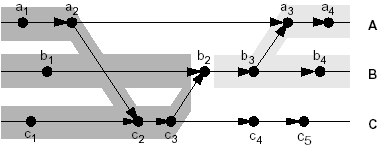
\includegraphics[width=0.45\textwidth]{img/img5.jpg}
	
	\caption{Структура зависимостей  событий}
	\label{fig:spire08}
\end{figure}

Следуя по стрелкам от события к событию с учётом взаимодействий, мы приходим к событиям, зависящим от начального. В отличии от последовательной программы, не все события в будущем могут быть достигнуты с помощью такого обхода, т.е. не все события причинно-зависимы. Рассмотрим событие b2. Все события в светло-серой области зависят от b2, но c4 и c5 не могут быть достигнуты из b2, так они не зависят от b2. Все события в тёмно-серой области влияют на b2, но все события, следующие за a2 и c3 могут быть отброшены при поиске причин b2.
При анализе трасс процессов с помощью таких зависимостей следует учесть, что:
1. необходимо знать положение каждого события локально внутри процесса;
2. должно быть возможно определить связанные пары событий в разных процессах
Эти требования могут быть удовлетворены, если исследуемая система предоставляет соответствующую информацию о событиях с сохранением её в трассе. При обработке таких трасс достаточным критерием для соответствия двух событий одному и тому же сообщению является одинаковое количество «пишущих» событий в одном процессе и «читающих» - в другом. В других случаях, например, при перекрывающихся  сообщениях, необходимо фиксировать дополнительную информацию, которая может быть использована для сопоставления пар событий. Примером такой информации могут служить номера пакетов в коммуникационных протоколах.
Анализ зависимостей в компьютерных системах означает следование по связанным событиям из конкретной точки, которая представляет собой интересное (нежелательное) поведение системы. Все инструкции программы, являющиеся причиной данного события являются кандидатами на оптимизацию. В параллельных системах с большим количеством процессов такое ограничение по предшествующим событиям позволяет сконцентрироваться на основных моментах, что приводит к значительному снижению затрат на анализ. 
\subsubsection{Сбор данных}
Учитывая сложность реальной вычислительной системы, не представляется возможным предсказать поведение системы во времени с помощью теоретических изысканий. По этой причине в большинстве инструментов программирования отсутствуют средства «планирования производительности». А те инструменты, в которые включён анализ производительности, дают лучшие результаты при профилировании. Профилирование оказывает большую помощь при программировании последовательных программ, при этом используется подход, основанный на измерениях. Т.е. определяется момент входа и выхода из каждой подпрограммы, подсчитывается количество вызовов каждой подпрограммы. Мониторинг(непрерывный процесс наблюдения и регистрации параметров объек) делает шаг вперёд по отношению к простому измерению – маркеры событий вставляются в программный код в местах, предоставляющих определённый интерес, и достижение маркера может означать, что программа совершила определённые действия. С помощью этих средств программа может быть анализирована на разных уровнях абстракции, определяемых разметкой исходников.
\subsubsection{Время сбора данных}
Есть два разных подхода к определению моментов, когда информация о состоянии системы должна быть собрана профилировщиком. Традиционные методы используют временнОй подход, при котором информация непрерывно пишется по протоколу, схожему с медицинским оборудованием, или данные собираются с определённой частотой. Этот подход имеет право на жизнь при малой частоте сбора данных для получения общего вида поведения системы. Для получения информации о внутреннем поведении вычислительной системы необходима высокая частота сбора событий с одной стороны и длительный промежуток времени – с другой. При описанном подходе это приведёт к огромному потоку данных.
Событийный мониторинг позволяет уменьшить объём данных на несколько порядков. При этом на важных частях программы фиксируется больше событий, чем на остальных. Тем самым достигается необходимая пользователю картина о динамическом поведении системы. При этом подходе измерения выполняемой программы порождают компактный вид системы, отбрасывающий детали, ненужные для решения текущего вопроса.
\subsection{Технологии параллельного программирования}
Широкое распространение компьютеров  распределённой памятью определило и появление соответствующих систем программирования. Как правило, в таких системах отсутствует единое адресное пространство, и для обмена данными между параллельными процессами используется явная передача сообщений через коммуникационную среду. Отдельные процессы описываются с помощью традиционных языков программирования, а для организации их взаимодействия вводятся дополнительные функции. По этой причине практически все системы программирования, основанные на явной передачи сообщений, существуют не только в виде новых языков, а в виде интерфейсов и библиотек.
К настоящему времени примеров известных систем программирования на основе передачи сообщений накопилось довольно много: Shmem, Linda, PVM, MPI, PARMACS, P4, MPL, NX и др. В этом разделе рассмотрим наиболее популярные системы.
\subsubsection{Linda}
Идея построения системы Linda исключительно проста, а потому красива и очень привлекательна. Параллельная программа есть множество параллельных процессов, и каждый процесс работает согласно обычной последовательной программе. Все процессы имеют доступ к общей памяти, единицей хранения в которой является кортеж. Отсюда происходит и специальное название для общей памяти - пространство кортежей. Каждый кортеж это упорядоченная последовательность значений. 
\subsubsection{PVM (Parallel Virtual Machine)}
Параллельную виртуальную машину (PVM) можно определить как часть средств реального вычислительного комплекса (процессоры, память, периферийные устройства и т.д.), предназначенную для выполнения множества задач, участвующих в получении общего результата вычислений. В общем случае число задач может превосходить число процессоров, включенных в PVM.
\subsubsection{MPI (Message Passing Interface)}
Наиболее распространённой технологией программирования параллельных компьютеров м распределённой памятью в настоящее время является MPI. Стандарт MPI фиксирует интерфейс, который должны соблюдать как система программирования MPI на каждой вычислительной системе, так и пользователь при создании свих программ. Современные реализации чаще всего соответствуют стандарту MPI версии 1.1. В 1997-1998 годах появился стандарт MPI 2.0, значительно расширяющий функциональность предыдущей версии. Однако, до сих пор этот стандарт не получил широкого распространения.
MPI-программа – это множество параллельных взаимодействующих процессов. Все процессы порождаются один раз, образуя параллельную часть программы. В ходе выполнения MPI-программы порождение дополнительных процессов или уничтожение существующих не допускается.
Каждый процесс работает в своём адресном пространстве, никаких общих переменных или данных в MPI нет. Основным способом взаимодействия между процессами является явная посылка сообщений. Для локализации взаимодействий параллельных процессов программы можно создавать группы процессов, предоставляя им общую среду для общения – коммуникатор. Состав образуемых групп произволен. Группы могут полностью входить одна в другую, не пересекаться или пересекаться частично. При старте программы всегда считается, что все порождённые процессы работают в рамках всеобъемлющего коммуникатора. Этот коммуникатор существует всегда и служит для взаимодействия всех процессов MPI-программы.
Каждый процесс имеет уникальный атрибут номер процесса, который является целым неотрицательным числом. С помощью этого атрибута происходит значительная часть взаимодействия процессов между собой. 
\section{Технология сбора данных}
Первостепенную важность для оценки эффективности параллельной программы имеет информация о взаимодействиях между её отдельными частями (процессами) и долях времён, затраченных процессами на взаимодействие и ожидание. Для  получения этой информации во время выполнения программы вызовы примитивов взаимодействия должны соответствующим образом обрабатываться средством трассировки. Рассмотрим основные подходы.
\subsection{Синтаксический анализ исходных текстов} С помощью синтаксического анализатора в исходном тексте программы выявляются вызовы примитивов взаимодействия и заменяются вызовами профилирующей библиотеки. Основным преимуществом этого метода является возможность для каждого вызова передать трассировщику положение этого вызова в исходном тексте, имена переменных и другую информацию, не доступную во время выполнения. В результате чего, при анализе трассы программы можно будет легко сопоставить вызовы библиотеки передачи сообщений с исходным кодом. Также есть возможность легко вернуться к «рабочему» варианту программы, без трассирующих вызовов, т.е. не использовать разбор кода. Из недостатков следует выделить: сложность реализации, зависимость от языка программирования, дополнительный шаг компиляции, увеличение объёма трассы.
\subsection{Статическое связывание с библиотекой профилировщика} В этом случае изменения исходного кода не требуются. Вместо этого на этапе связывания вызовы библиотеки передачи сообщений подменяются вызовами профилировщика. Конфликт имён при этом разрешается либо за счёт многоэтапного связывания, либо за счёт «слабых» (week) связей. Как и в предыдущем случае, здесь не требуется вносить изменения в исходный код, но при этом не требуется проводить сложный анализ исходного кода.
\subsection{Определение точек трассировки во время выполнения} Метод основан на анализе частоты и шаблонов вызовов функций во время выполнения программы. При этом двоичный код программы компилируется стандартным образом, а профилирующие вызовы вставляются автоматически на основе реального поведения программы. Этот метод можно использовать при невозможности перекомпиляции программы. Но придётся столкнуться с такими проблемами как: зависимость от конкретной платформы, отсутствие возможности прямо указать необходимость профилирования того или иного участка программы, сложность сопоставления обнаруженного узкого места с исходным кодом.
Кроме получения информации о системных вызовах программы, также необходимо предоставить пользователю возможность указывать собственные временнЫе метки. Это позволяет определить время выполнения логических участков программы, а также упростить связь событий трассы с исходным кодом.
Работа над выявлением узких мест в программе как правило ведётся итерационно, со всё большим уровнем детализации. При этом внимание разработчика сосредотачивается на отдельных участках программы, оставляя другие участки за кадром. Чтобы снизить объём трассы, средство трассировки должно допускать трассировку только части программы, иметь средства для приостановки и возобновления трассировки \cite{book3}.
Изложенным требованиям удовлетворяет библиотека PICL, использующая для трассировки интерфейс профилирования MPI.
\section{PICL}
PICL (Portable Instrumented Communication Library)  - библиотека подпрограмм, разработанная в Oak Ridge National Laboratory (ORNL), которая реализует общий
нтерфейс передачи сообщений на множестве многопроцессорных архитектур. Программы, написанные с помощью примитивов PICL вместо команд среды взаимодействия, являются переносимыми в том смысле, что они могут выполняться на любой машине, для которой есть реализация PICL.\\
PICL была разработана для:
\begin{enumerate} 
	\item Обеспечения переносимости между разными платформами с минимальными накладными расходами;
	\item Получения трассировочных данных по межпроцессным взаимодействиям и пользовательским событиям, также с минимальными накладными расходами для избежания влияния на поведение исследуемой задачи, и
	\item Обеспечения переносимости на новые системы, простого расширения для использования преимуществ новых команд конкретной системы
\end{enumerate} 
Для достижения этих целей PICL реализована как библиотека подпрограмм языка C с машинно-независимым трассировочным слоем и машинно-зависимым слоем, отображающимся на команды конкретной системы (когда это возможно). PICL  была открыта для широкого использования в марте 1989. Её разработка продолжалась, и были выпущены несколько релизов, добавляющие новые коммуникационные и трассировочные команды и поддержку новых вычислительных систем.
В последней версии PICL запись трассы имеет формат, показанный в таблице \ref{tab:tbl1}. Для каждой записи обязательными являются первые шесть полей, но если количество полей данных равно нулю, то дескриптор данных исключается.

\begin{table}[h!]
	\caption{\label{tab:tbl1}Формат записи трассы PICL}
	\begin{tabular}{|l|l|}
		%	&\makebox[3em]{6/3}&\makebox[3em]{6/4}
		\hline
		Наименование поля & Назначение \\
		\hline\hline
		тип записи&тип информации в записи
		\\\hline
		тип события &тип события, с которым связана запись
		\\\hline
		отметка времени&когда информация была истинной\\\hline
		идентификатор процессора
		&процессор, с которым связана информация
		\\\hline
		идентификатор процесса	
		&процесс, с которым связана информация	
		\\\hline
		количество полей данных	
		&количество дополнительных полей данных, связанных \tabularnewline & с данными типами записи и события	
		\\\hline
		дескриптор данных	
		&формат полей данных
		\\\hline
		данные	
		&дополнительные поля данных
		\\\hline
		
	\end{tabular}
\end{table}
Основное внимание в этом формате уделено записи информации, связанной как с системными, так и с пользовательскими событиями, при этом каждая запись связана с определённым типом события. Порядок полей записи отражает важность полей для систем, обрабатывающих данные: что, где, когда и ассоциированные с событием данные. Если тип записи или события не знаком системе, то данную запись можно пропустить. Но если система хочет получить информацию из записи, то ей для этого всё предоставлено.

Формат PICL предусматривает ранение данных в текстовом виде. Все поля состоят из символов кодировки ASCII и разделены пробелами. Тип записи, тип события, идентификаторы процессора и процесса, количество полей данных – целые числа. Дескриптор данных – это либо целое число, либо символьная строка переменной длины, заключённая в двойные кавычки. Формат полей данных определяется дескриптором данных. Временная метка – число с плавающей точкой, разрешение которой зависит от единиц измерения (например, секунд) и точности таймера на машине, на которой генерируется трасса.

Практика показала, что текстовый формат очень полезен для переносимости, поиска и исправления ошибок в трассе и для возможной работы с трассой без помощи средств визуализации, и он не препятствует сжатию файлов, если это необходимо. При этом PICL использует двоичное представление данных при внутренней обработке для экономии места и избежания накладных расходов при преобразовании данных \cite{book4}.
Значения полей и их интерпретация приведены в таблице \ref{tab:tbl2}
\begin{table}[h!]
	\caption{\label{tab:tbl2} Значения полей записи}
	\begin{tabular}{|l|l|}
		%	&\makebox[3em]{6/3}&\makebox[3em]{6/4}
		\hline
		Поле & Назначение \\
		\hline\hline
		тип записи& $\geq0$ пользовательский тип записи\tabularnewline & $\le0$ стандартный системный тип записи
		\\\hline
		тип события & $\geq0$ пользовательское событие или определённое \tabularnewline & пользователем подмножество событий\tabularnewline & $=-1$ относится ко всем событиям \tabularnewline &(глобальная информация)
		\tabularnewline & $<-1$ системное событие или \tabularnewline &системное подмножество событий
		\\\hline
		временная метка& $\geq0$идентификатор конкретного процессора\tabularnewline & $=-1$ относится ко всем процессорам \tabularnewline &(глобальная информация)
		\tabularnewline & $<-1$ относится к подмножеству процессоров
		\\\hline
		идентификатор процесса
		&$\geq0$ идентификатор процесса\tabularnewline & на заданном процессоре\tabularnewline & $=-1$ относится ко всем процессам\tabularnewline & на заданном процессоре \tabularnewline &(глобальная информация)
		\tabularnewline & $<-1$ относится к подмножеству процессов\tabularnewline & на указанном процессоре
		\\\hline
		количество полей данных	
		&количество дополнительных полей данных	
		\\\hline
		дескриптор данных
		& если заключён в двойные кавычки,\tabularnewline & то формат функции scanf(),
		иначе:\tabularnewline &
		$=0$  символ ("\%c") \tabularnewline & $=1$ cтрока ("\%s") \tabularnewline &
		$=2$ целое число ("\%d") \tabularnewline &
		$=3$ длинное целое число  ("\%ld") \tabularnewline &
		$=4$ число с плавающей точкой одинарной точности  ("\%f") \tabularnewline &
		$=5$ число с плавающей точкой двойной точности   ("\%lf") \tabularnewline &
		$>6$ другой предопределённый формат данных \tabularnewline &
		
		
		\\\hline
		
	\end{tabular}
\end{table}
Идентификаторы процесса и процессора определяют «местоположение» события. Хотя обычно процессы на каждом процессоре нумеруются последовательно начиная с 0, может быть полезно нумеровать процессы независимо от процессора, прямо поддерживая как процессоро-зависимый, так и процессоро-независимый подход к визуализации. (Заметим, что на данный момент PICL не поддерживает много процессов на одном (последовательном) процессоре. Поле идентификатора процесса было введено для совместимости с системами, которые поддерживают эту модель и для возможности будущего расширения PICL. В трассах текущего формата идентификатору процесса присваивается либо действительной PID, т.е. номер процесса, заданный операционной системой, либо -1.

%%% Local Variables:
%%% mode: latex
%%% TeX-master: "rpz"
%%% End:

\chapter{Конструкторский раздел}
\label{cha:design}
\section{Общая архитектура приложения}
\begin{figure}[h!]
	\centering
	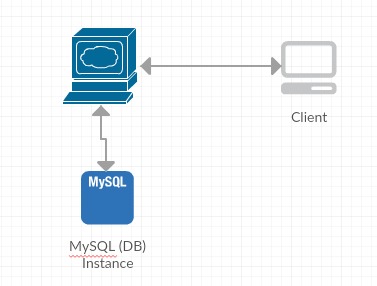
\includegraphics[width=0.6\textwidth]{img/img5.png}
	\caption{Общая архитектура приложения}
	\label{fig:spire09}
\end{figure}
Приложение построено по архитектуре "клиент-сервер". Клиент запускает на своём компьютере приложение и взаимодействует посредством сети с удаленным сервером. Сервер позволяет осуществлять доступ к необходимой информации из базы данных, разграничивать доступ пользователей к той или иной информации. Так же на сервере находится приложение, позволяющее парсить trace-файлы программы и заносить информацию в базу данных.
)

\section{Клиентская часть}
Клиентское приложение позволяет осуществлять авторизацию, получать информацию о доступном ему списке файлов трасс, получать общую информацию о файле трасс, получать детальную информацию о файле трасс в заданном временом временном интервале с заданным количеством процессов.
\begin{figure}[h!]
	\centering
	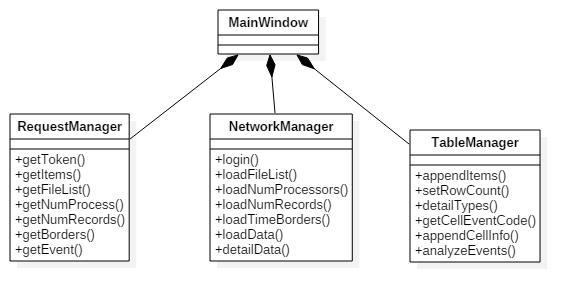
\includegraphics[width=0.8\textwidth]{img/client.png}
	\caption{Диаграмма классов клиентского приложения}
	\label{fig:spire10}
\end{figure}
\\ \textbf{MainWindow.} Класс графического интерфейса приложение. Реализует логику взаимодействия между клиентом и программой.\\
\textbf{NetworkManager.} Класс работы с сетью. Реализует логику асинхронных запросов к серверу.\\
\textbf{RequestManager.} Класс работы с телами ответов сервера.Парсит приходяющую с сервера информацию. \\
\textbf{TableManager.} Класс работы с визуалиацией приходящей информации. Реализует логику работы с таблицей отображения trace-информации.
\section{Серверная часть}
Сервер был разработан на базе NodeJS express. Он позволяет асинхронно работать с поступающим ему запросами. Код сервера представляет собой множество функций-обработчиков приходящих запросов.
\begin{lstlisting}[language=c++]
apiRoutes.get('/authenticate', function (req, res) {..}
apiRoutes.get("/getFile", function (req, res) {...}
apiRoutes.get("/getTimeBorders", function (req, res) {...}
apiRoutes.get("/getFileList", function (req, res) {...}
apiRoutes.get("/getNumRecords", function (req, res) {...}
apiRoutes.get("/getCodeInfo", function (req, res) {...}
apiRoutes.get("/getNumProcesses", function (req, res) {...}
\end{lstlisting}

\subsection{API для взаимодействия с сервером}
Была разработано API взаимодействия между клиентом и сервером. Безопастность взаимодействия гарантируется тем, что взаимодействия осуществляется на основе токенов. Все запросы, кроме запроса на авторизацию, требуют содержания в себе уникального токена.Токен дается клиенту после успешного прохождения авторизации. 
\begin{lstlisting}[language=c++]
(*\bfseries [GET] /authenticate *)
Авторизация
Аргументы
)name - логин
)password - пароль

(*\bfseries [Example response]*)
{
"success": true,
"message": "Enjoy your token!",
"token": "eyJhbGciOiJIUzI1NiIsInR5cCI6IkpXVCJ9.eyJ1c2VyIj
oiVXNlciIsInBhc3N3b3JkIjoicHdkI
iwiaWF0IjoxNDk2NDM4ODc4LCJleHAiOjE0OT
Y1MjUyNzh9.0bhg6Ct8YXOGixVY-ZukmdVj
-35AE0BSZExGWJlpNKQ"
}

(*\bfseries[GET] /getFile*)
Получение куска содержанимого файла
Аргументы
)filename - имя файла
)offset - отступ от начала файла
)limit - количество получаемых записей
)timeMin - время начала записей
)timeMax - время конца записей

(*\bfseries [Example response]*)
{
"result": [
{
"filename": "trace1",
"typeRecord": -3,
"typeEvent": -901,
"time": 0.000007,
"prid": 0,
"pid": 0,
"numData": 0,
"data": "-1"
}],
}

(*\bfseries[GET] /getTimeBorders*)
Получение временного интервала трассы
Аргументы
)filename - имя файла

(*\bfseries [Example response]*)
{
"result": [
{
"MIN(time)": 0.000007000000096013537,
"MAX(time)": 0.11629900336265564
}],
}

(*\bfseries[GET] /getFileList*)
Получение списка файлов, доступных для данного пользователя
Аргументы
)name - логин

(*\bfseries [Example response]*)
{
"success": true,
"message": [
{
"filename": "trace1"
},
{
"filename": "trace2"
}],
}

(*\bfseries[GET] /getNumRecords*)
Получение количества записей для данного файла
Аргументы
)filename - имя файла
)timeMin - время начала записей
)timeMax - время конца записей
 
 (*\bfseries [Example response]*)
 {
 "result": [
 {
 "COUNT": 522
 }],
 }
 
(*\bfseries[GET] /getCodeInfo*)
Получение информации о событие по его коду
Аргументы
)code - код события

(*\bfseries [Example response]*)
{
"result": [
{
"name": "WILDCARD",
"description": "wildcard for all or any processes",
"category": "event type definitions"
}],
}

(*\bfseries[GET] /getNumProcess*)
Получение максимального количества процессов, которые записаны в файл
Аргументы
)filename - имя файла

(*\bfseries [Example response]*)
{
"result": [
{
"max(prid)": 7
}],
}
\end{lstlisting}
\section{Взаимодействие клиента и сервера}
\begin{figure}[h!]
	\centering
	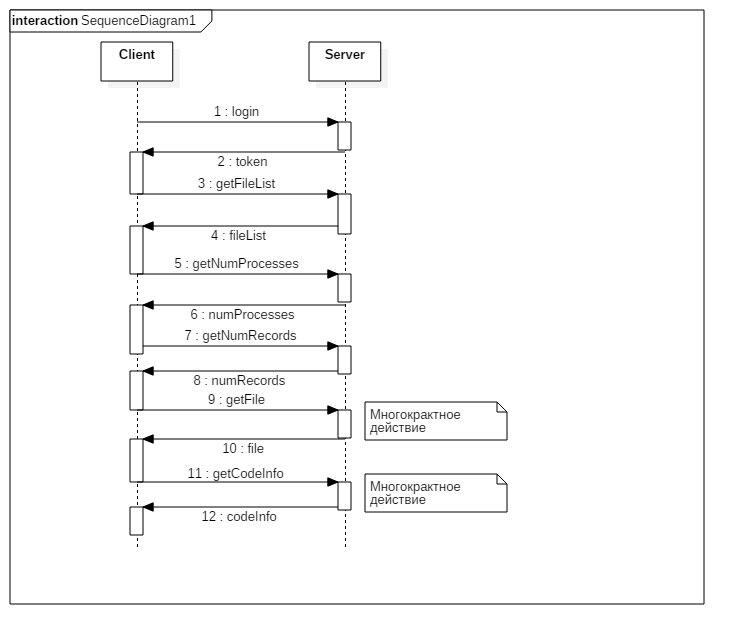
\includegraphics[width=1.1\textwidth]{img/clientServer.jpg}
	\caption{Диаграмма взамодействия клиента и сервера}
	\label{fig:spire12}
\end{figure}
В начале работы приложения клиент должен пройти авторизацию(1). В случае успешного прохождения авторизации ему посылается token,позволяющий ему получить права доступа к работе с trace-информацией(2). После этого клиент загружает список доступных ему файлов(3-4).
Запросы (5-8) технические и нужны для корректного отображения trace-информации на стороне клиента.  После того как вся техническая информация была загружена, клиент приступает к загрузке файла(9-10). Файл загружается <<небольшими порциями>>, поэтому возможно многократное повторение запросов (9-10) до успешной загрузки файла. В случае успешной загрузки файла клиент может получить детальную информацию об этом файле при помоще запросов (11-12).
\section{Синтаксический анализ trace-файлов}
Для синтаксического анализа(парсинга) trace-файлов и занесения их в базу данных была разработана консольная программа.
\begin{figure}[h!]
	\centering
	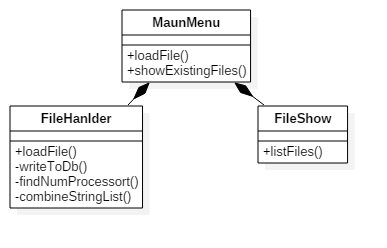
\includegraphics[width=0.6\textwidth]{img/server.png}
	\caption{Диаграмма классов серверного приложения}
	\label{fig:spire11}
\end{figure}
\\ \textbf{MainMenu.} Класс главного меню программы. Реализует логику взаимодействия между клиентом и программов. \\
\textbf{FileShow.} Класс для работы с файловой системой компьютера. \\
\textbf{FileHandler.} Класс для парсинга trace-файла. Реализует логику анализа trace-файла и занесения его в базу данных.
\section{Базы данных}
Для хранения файлов трасс формата PICL была спроектирована база данных.
\begin{lstlisting}[language=SQL]
CREATE TABLE Tracks ( 
filename VARCHAR(50) NOT NULL,
typeRecord INT NOT NULL,
typeEvent INT NOT NULL,
time FLOAT NOT NULL,
prid INT NOT NULL,
pid INT NOT NULL,
numData INT NOT NULL,
data VARCHAR(200),
FOREIGN KEY (typeEvent) REFERENCES Codes(code) 
ON DELETE CASCADE ON UPDATE CASCADE,
FOREIGN KEY (filename) REFERENCES Files(filename) 
ON DELETE CASCADE ON UPDATE CASCADE
) ENGINE = INNODB DEFAULT CHARSET=utf8;
\end{lstlisting}
Так же были спроектирована вспомогательные базы данных для хранения информации о событиях MPI, файлах, пользователях.
\begin{lstlisting}[language=SQL]
CREATE TABLE Users(
user  VARCHAR(50) NOT NULL  PRIMARY KEY,
password  VARCHAR(50) NOT NULL
) ENGINE = INNODB DEFAULT CHARSET=utf8;

CREATE TABLE Files(
filename  VARCHAR(50) NOT NULL PRIMARY KEY
) ENGINE = INNODB DEFAULT CHARSET=utf8;

CREATE TABLE FilesUsers(
user  VARCHAR(50) NOT NULL,
filename  VARCHAR(50) NOT NULL,
PRIMARY KEY (user, filename), 
FOREIGN KEY (filename) REFERENCES Files(filename)
ON DELETE CASCADE ON UPDATE CASCADE 
) ENGINE = INNODB DEFAULT CHARSET=utf8;

CREATE TABLE Codes(
code  INT NOT NULL  PRIMARY KEY,
name  VARCHAR(50) NOT NULL,
description TEXT,
category TEXT
) ENGINE = INNODB DEFAULT CHARSET=utf8;

\end{lstlisting} 

\subsection{Нормальные формы}
Нормальная форма — свойство отношения в реляционной модели данных, характеризующее его с точки зрения избыточности, потенциально приводящей к логически ошибочным результатам выборки или изменения данных. Нормальная форма определяется как совокупность требований, которым должно удовлетворять отношение.
Процесс преобразования отношений базы данных (БД) к виду, отвечающему нормальным формам, называется нормализацией. Нормализация предназначена для приведения структуры БД к виду, обеспечивающему минимальную логическую избыточность, и не имеет целью уменьшение или увеличение производительности работы или же уменьшение или увеличение физического объёма базы данных. Конечной целью нормализации является уменьшение потенциальной противоречивости хранимой в базе данных информации. Как отмечает К. Дейт, общее назначение процесса нормализации заключается в следующем:
\begin{enumerate}

	\item исключение некоторых типов избыточности;
	\item устранение некоторых аномалий обновления;
	\item разработка проекта базы данных, который является достаточно «качественным» представлением реального мира, интуитивно понятен и может служить хорошей основой для последующего расширения;
	\item упрощение процедуры применения необходимых ограничений целостности.

\end{enumerate}
Устранение избыточности производится, как правило, за счёт декомпозиции отношений таким образом, чтобы в каждом отношении хранились только первичные факты (то есть факты, не выводимые из других хранимых фактов)\cite{book6}.

\textbf{Первая нормальная форма}. Переменная отношения находится в первой нормальной форме тогда и только тогда, когда в любом допустимом значении отношения каждый его кортеж содержит только одно значение для каждого из атрибутов.
В реляционной модели отношение всегда находится в первой нормальной форме по определению понятия отношение.
Что же касается различных таблиц, то они могут не быть правильными представлениями отношений и, соответственно, могут не находиться в 1NF. В соответствии с определением К. Дж. Дейта для такого случая, таблица нормализована (эквивалентно — находится в первой нормальной форме) тогда и только тогда, когда она является прямым и верным представлением некоторого отношения. Конкретнее, рассматриваемая таблица должна удовлетворять следующим пяти условиям:
\begin{enumerate}
\item Нет упорядочивания строк сверху-вниз (другими словами, порядок строк не несет в себе никакой информации).
\item Нет упорядочивания столбцов слева-направо (другими словами, порядок столбцов не несет в себе никакой информации).
\item Нет повторяющихся строк.
\item Каждое пересечение строки и столбца содержит ровно одно значение из соответствующего домена.
\item Все столбцы являются обычными (в таблице нет «скрытых» компонентов, которые могут быть доступны только в вызове некоторого специального оператора взамен ссылок на имена регулярных столбцов).
\end{enumerate}
В моей базе данных каждый кортеж всех таблиц содержит только атомарные атрибуты (атрибут атомарен, если его значение теряет смысл при любом разбиении на части или переупорядочивании), отсутствуют повторяющиеся кортежи. Исходя из этого, можно сказать, что все таблицы находятся в первой нормальной форме.

\textbf{Вторая нормальная форма}. Переменная отношения находится во второй нормальной форме тогда и только тогда, когда она находится в первой нормальной форме и каждый неключевой атрибут неприводимо зависит от её потенциального ключа.
Неприводимость означает, что в составе потенциального ключа отсутствует меньшее подмножество атрибутов, от которого можно также вывести данную функциональную зависимость. Для неприводимой функциональной зависимости часто используется эквивалентное понятие «полная функциональная зависимость». Если потенциальный ключ является простым, то есть состоит из единственного атрибута, то любая функциональная зависимость от него является неприводимой (полной). Если потенциальный ключ является составным, то согласно определению второй нормальной формы в отношении не должно быть неключевых атрибутов, зависящих от части составного потенциального ключа.
Вторая нормальная форма по определению запрещает наличие неключевых атрибутов, которые вообще не зависят от потенциального ключа. Таким образом, вторая нормальная форма запрещает создавать отношения как несвязанные (хаотические, случайные) наборы атрибутов.
В моей базе данных не все потенциальные ключи состоят из одного атрибута, следовательно, нельзя сказать, что все таблицы находятся во второй нормальной форме.

%%% Local Variables:

%%% mode: latex
%%% TeX-master: "rpz"
%%% End:
%--количество цветов
%||количество пикселей
\chapter{Технологический раздел}
\section{Выбор  языка программирования}
Для реализации  был выбран язык  С++. Данный язык был обоснован следующими причинами:
Причины:
\begin{enumerate}
	 \item Его поддерживает библиотека PICL
	 \item Компилируемый язык со статической типизацией. 
	 \item Сочетание высокоуровневых и низкоуровневых средств.
	 \item Реализация ООП.
	 \item Наличие удобной стандартной библиотеки шаблонов
	 \end{enumerate}
\section{Выбор вспомогательных библиотек}
Для реализации программы была выбрана библиотека Qt.
\begin{enumerate}
	\item Широкие возможности работы с изображениями, в том числе и попиксельно
	\item Наличии более функциональных аналогов стандартной библиотеки шаблонов в том числе для разнообразных структур данных
\end{enumerate}
Так же были были использованы библиотеки Nodejs,express,jsonwebtoken,mysql-nodejs,mongoose/
\section{Выбор базы данных}
Для хранения файлов трасс была выбрана база данных MySQL
\begin{enumerate}
	\item Быстродействие. Благодаря внутреннему механизму многопоточности быстродействие MySQL весьма высоко.
	\item Лицензия. Раньше лицензирование MySQL было немного запутанным; сейчас эта программа для некоммерческих целей распространяется бесплатно
	\item Переносимость. В настоящее время существуют версии программы для большинства распространенных компьютерных платформ. Это говорит о том, что вам не навязывают определенную операционную систему. Вы сами можете выбрать, с чем работать, например с Linux или Windows, но даже в случае замены ОС вы не потеряете свои данные и вам даже не понадобятся дополнительные инструменты для их переноса.
\end{enumerate}
Для хранения базы данных логинов и паролей была выбрана NoSQL документориентированная база данных MongoDB.
\begin{enumerate}
	\item Быстрое извлечение простых структур данных \cite{book5}.
	\item Может хранить неструктурную информацию
	 \item Лицензия. Для некоммерческих целей распространяется бесплатно.
\end{enumerate}



%%% Local Variables:
%%% mode: latex
%%% TeX-master: "rpz"
%%% End:

\chapter{Исследовательский раздел}
%\chapter{Заключение}
\label{cha:research}
\section{Время дизеринга раличных алгоритмов}

%В данном разделе проводятся вычислительные эксперименты.
Рассмотрим время работы различных алгоритмов для различных размеров изображения.

\begin{tabular}{|@{\hspace*{2mm}}l||*{3}{c|}}\hline

	&\makebox[12em]{Размер, пиксели}&\makebox[6em]{Время, мкс}
	%	&\makebox[3em]{6/3}&\makebox[3em]{6/4}
	\\\hline\hline
	White noise&133x90&862\\\hline
	Blue noise&133x90&930\\\hline
	Brown noise&133x90&934\\\hline
	Violet noise &133x90&937\\\hline
	Pink noise noise&133x90&930\\\hline
	Floyd-SD&133x90&1200\\\hline
	F. Floyd-SDe&133x90&1093\\\hline
	JJN &133x90&1909\\\hline
	White noise&458x458&15735\\\hline
	Blue noise&458x458&19374\\\hline
	Brown noise&458x458&19432\\\hline
	Violet noise &458x458&18787\\\hline
	Pink noise noise&458x458&18129\\\hline
	Floyd-SD&458x458&27173\\\hline
	F. Floyd-SDe&458x458&26424\\\hline
	JJN &458x458&47201\\\hline
	White noise&458x458&194376\\\hline
	Blue noise&458x458&200577\\\hline
	Brown noise&458x458&208400\\\hline
	Violet noise &458x458&251294\\\hline
	Pink noise noise&458x458&258775\\\hline
	Floyd-SD&458x458&251294\\\hline
	F. Floyd-SDe&458x458&387104\\\hline
	JJN &458x458&857481\\\hline
\end{tabular}
\bigskip
\\
Из рассмотрения вынесены алгоритм Юлиомы в вследствие того, что он значительно медленней других алгоритмов(2732568 мкс для изображения 113х90) в и алгоритм Байера, реализованный при помощи шейдеров, вследствии того, что он не не укладывается в рамки требуемой палитры (при этом он работает очень быстро 64 мс для изображени 640х480).
\section{Качество получаемого изображения}
\begin{tabular}{|@{\hspace*{2mm}}l||*{3}{c|}}\hline
	
	&\makebox[15em]{PSNR}&\makebox[6em]{SSIM}
	%	&\makebox[3em]{6/3}&\makebox[3em]{6/4}
	\\\hline\hline
	White noise&33.2894&0.914778\\\hline
	Blue noise& 36.1756&0.971626\\\hline
	Brown noise&33.32370&0.915767\\\hline
	Violet noise &37.63480&0.984574\\\hline
	Pink noise &36.4484&0.974718\\\hline
	Floyd-SD& 37.0553&0.979173\\\hline
	F. Floyd-SDe&36.8401&0.976452\\\hline
	JJN &37.30740&0.981688\\\hline
	Yliouma&36.2359&0.967796\\\hline
	Without dithering&37.6348&0.984574\\\hline
\end{tabular}
\bigskip
\\
Несмотря на то, что некоторые сложные алгоритмы дизеринга диффузии ошибок обещат получения хорошего качества изображений,некоторые алгоритмы случайного дизеринга на конкретных изображениях дают лучший результат. Для того чтобы получить наилучший результат дизеринга, следует проанализировать результаты дизеринга нескольких изображений и выбрать среди них наилучшее.
Так же следует отметить некоторую необъективность метрик: результат метрик не всегда совпадает с человеческим восприятием картинки.
%\begin{figure}
 % \centering
 % \caption{Как страшно жить}
 % \label{fig:spire01}
%\end{figure}
\section{Размер получаемого изображения}

\begin{tabular}{|@{\hspace*{2mm}}l||*{3}{c|}}\hline
	
	&\makebox[8em]{Разрешение, пикс}&\makebox[5em]{Размер, кб} &\makebox[7em]{Исх. раз., кб}
	%	&\makebox[3em]{6/3}&\makebox[3em]{6/4}
	\\\hline\hline
	White noise&900x675&186&\multirow{6}{*}{2373 bmp,1779 png} \\\cline{1-3}
	Blue noise& 900x675&135& \\\cline{1-3}
	Brown noise&900x6750&186&\\\cline{1-3}
	Violet noise &900x675&98&\\\cline{1-3}
	Pink noise &900x675&1158&\\\cline{1-3}
	Floyd-SD& 900x675&1273&\\\cline{1-3}
	F. Floyd-SDe&900x675&143&\\\cline{1-3}
	JJN &900x675&117&\\\hline
	White noise&3984х32355&3431&\multirow{6}{*}{50344 bmp,37758 png} \\\cline{1-3}
	Blue noise& 3984х3235&2570& \\\cline{1-3}
	Brown noise&3984х3235&3432&\\\cline{1-3}
	Violet noise &3984х3235&1950&\\\cline{1-3}
	Pink noise &3984х3235&2406&\\\cline{1-3}
	Floyd-SD& 3984х32355&3605&\\\cline{1-3}
	F. Floyd-SDe&3984х3235&4269&\\\cline{1-3}
	JJN &3984х3235&3716&\\\hline
\end{tabular}
\bigskip
\\

Из вышеприведенной таблицы, можно заметить, размер изображения после дизеринга значительно уменьшиается,достирается выигрыш в размере изображение до 15 раз, в зависимости от иходного контейнера изображения и выбранного способра дизеринга.
%%% Local Variables:
%%% mode: latex
%%% TeX-master: "rpz"
%%% End:

%\chapter{Организационно-экономический раздел}
%\label{cha:econom}
%%% Local Variables:
%%% mode: latex
%%% TeX-master: "rpz"
%%% End:

%\chapter{Промышленная экология и %езопасность}\label{cha:bzd}


%%% Local Variables:
%%% mode: latex
%%% TeX-master: "rpz"
%%% End:


\backmatter %% Здесь заканчивается нумерованная часть документа и начинаются ссылки и
            %% заключение

\Conclusion % заключение к отчёту

\begin{figure}
В данной работе были реализованы различные алгоритмы дизеринга, было произведено сравнение и анализ этих алгоритмов. Программа позволяет получить изображение схожего визуального качества при значительном уменьшении размера. Был получен вывод о том, что для различных целей следует использовать различные алгоритмы дизеринга, универсального алгоритма дизеринга не существует. Программа не привязана к какой-то конкретной
операционной системе и может быть скомпилирована и запущена на
всех популярных ОС.
\end{figure}
%%% Local Variables: 
%%% mode: latex
%%% TeX-master: "rpz"
%%% End: 


% % Список литературы при помощи BibTeX
% Юзать так:
%
% pdflatex rpz
% bibtex rpz
% pdflatex rpz

\bibliographystyle{gost780u}
\bibliography{rpz}


%%% Local Variables: 
%%% mode: latex
%%% TeX-master: "rpz"
%%% End: 


\appendix   % Тут идут приложения

%\chapter{Картинки}
%\label{cha:appendix1}

%\begin{figure}
%\centering
%\caption{Картинка в приложении. Страшная и ужасная.}
%\end{figure}

%%% Local Variables: 
%%% mode: latex
%%% TeX-master: "rpz"
%%% End: 

%\chapter{Еще картинки}
%\label{cha:appendix2}

%\begin{figure}
%\centering
%\caption{Еще одна картинка, ничем не лучше предыдущей. Но %надо же как-то заполнить место.}
%\end{figure}

%%% Local Variables: 
%%% mode: latex
%%% TeX-master: "rpz"
%%% End: 


\end{document}

%%% Local Variables:
%%% mode: latex
%%% TeX-master: t
%%% End:
